\documentclass{exam}

\usepackage{units} 
\usepackage{graphicx}
\usepackage[fleqn]{amsmath}
\usepackage{cancel}
\usepackage{float}
\usepackage{mdwlist}
\usepackage{booktabs}
\usepackage{cancel}
\usepackage{polynom}
\usepackage{caption}
\usepackage{fullpage}
\usepackage{xfrac}
\usepackage{enumerate}

\newcommand{\degree}{\ensuremath{^\circ}} 
\everymath{\displaystyle}

\printanswers

% \begin{figure}[H]
%   \centering
%   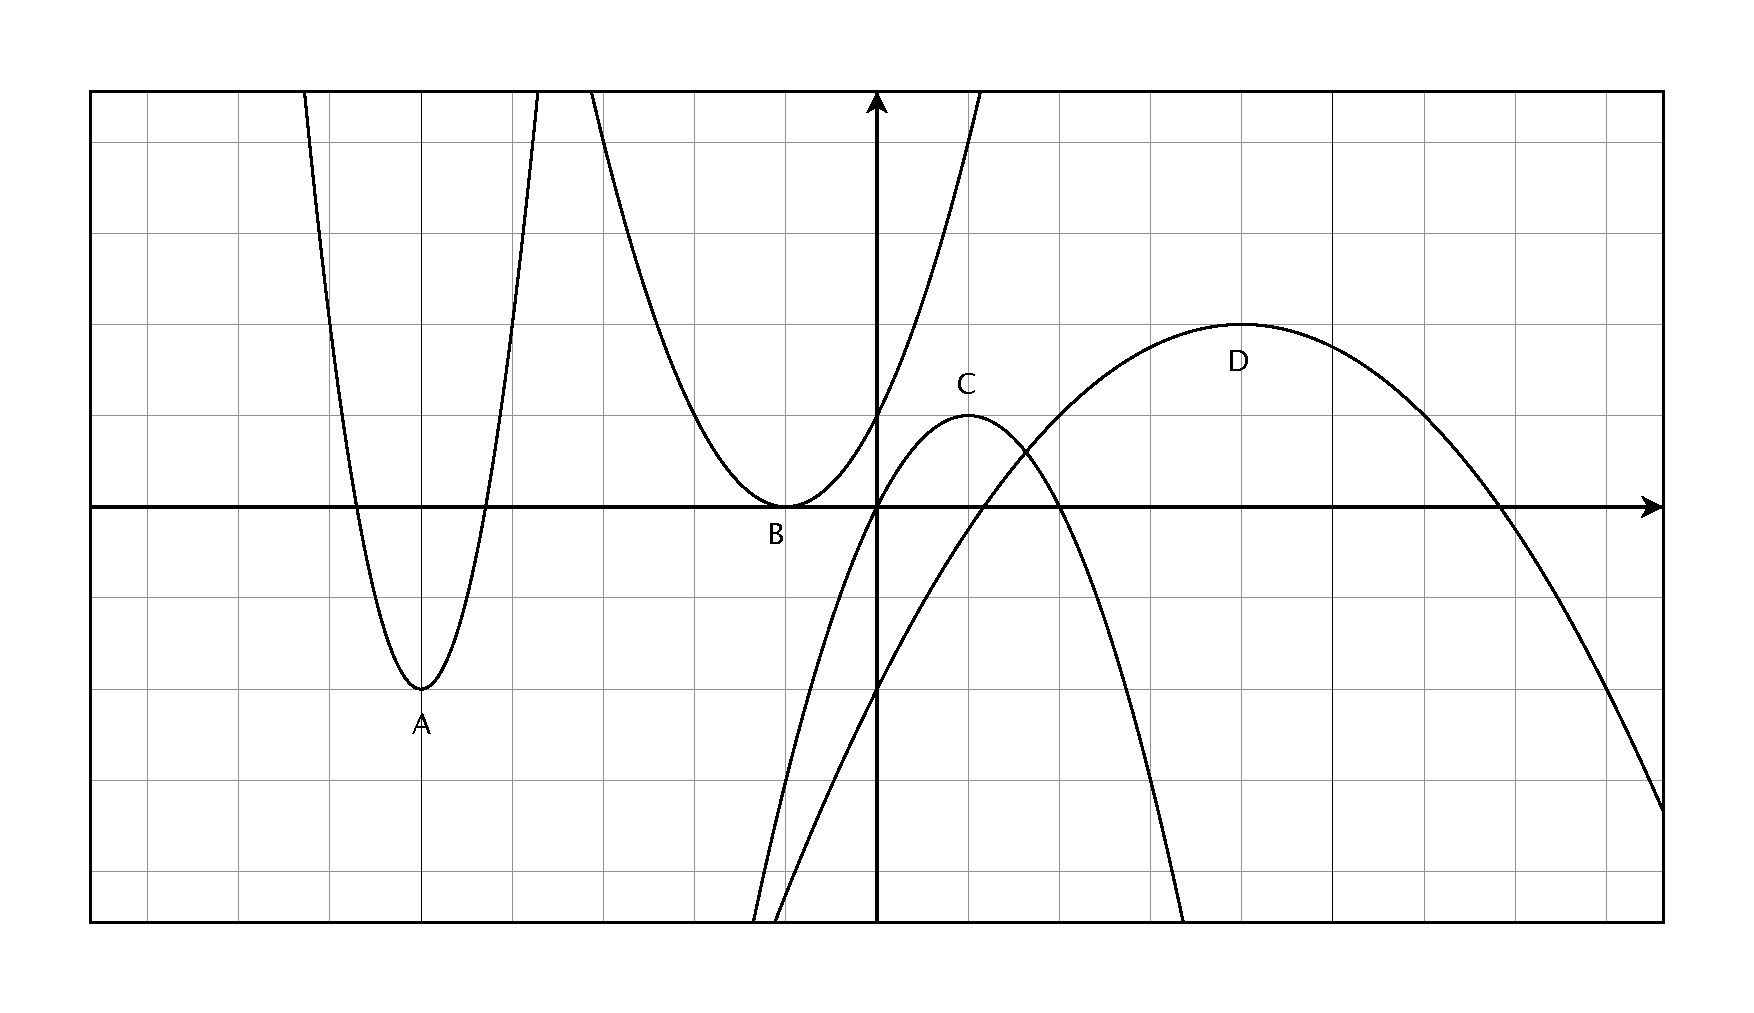
\includegraphics[scale=.3]{problem_7.eps}
%   \caption*{Problem 7}
% \end{figure}

% \begin{tabular}{cc}
% \toprule
% period & amplitude \\
% \midrule
%   $\pi$ & $2$ \\
% \bottomrule
% \end{tabular}

\title{Math 142 Notes \\ Section 5.4}

\date{\today}

\begin{document}

  \maketitle
  \tableofcontents

  \section{Homework}

  \begin{itemize*}
    \item If you don't do the homework, you'll end up lost.  It's very hard to catch up--if you don't do the homework
      each week, you'll end up dropping out.

    \item review odd/even

    \item do cotangent projection problem
  \end{itemize*}

  \section{Tangent/Cotangent Graphs}

  \subsection{Cotangent}

  \begin{itemize}
    \item Draw projection picture (extra credit question)
    \item Talk about airplane:
      \begin{itemize*}
        \item when far away, small change in angle leads to large change in position or large change in position
          provides only small change in position
        \item draw unit circle with equal intervals on circle
        \item draw unit circle with equal intervals on cotangent line.
        \item draw cotangent graph
        \item draw equal intervals on x-axis 
        \item draw equal intervals on y-axis
      \end{itemize*}
  \end{itemize}

  \begin{figure}[H]
    \centering
    \includegraphics{example01.eps}
    \caption{Cotangent}
  \end{figure}

  \subsection{Tangent}

  \begin{itemize}
    \item Draw projection picture (extra credit question)
    \item Talk about elevator:
      \begin{itemize*}
        \item when far away, small change in angle leads to large change in position or large change in position
          provides only small change in position
        \item draw unit circle with equal intervals on circle
        \item draw unit circle with equal intervals on cotangent line.
        \item draw cotangent graph
        \item draw equal intervals on x-axis 
        \item draw equal intervals on y-axis
      \end{itemize*}
  \end{itemize}

  \begin{figure}[H]
    \centering
    \includegraphics{example02.eps}
    \caption{Tangent}
  \end{figure}

  \section{Limits}
  \begin{align*}
    \lim_{t \to 0+} \cot t & = \infty \\
    \lim_{t \to 0-} \cot t & = -\infty \\
    \\
    \lim_{t \to \frac{\pi}{2}-} \tan t & = \infty \\
    \lim_{t \to \frac{\pi}{2}+} \tan t & = -\infty \\
  \end{align*}

  \begin{itemize}
    \item informally: as $t$ gets closer to 0 from the positive side, $\cot t$ gets progressively larger
    \item like a challenge: if you give me a positive number $k$, I can find a $\delta$ where as long as $t$ is between 0 and
      $\delta$, $\cot t$ will be greater than $k$.
  \end{itemize}

\end{document}
